\documentclass[]{article}
\usepackage{graphicx}
\usepackage[svgnames]{xcolor} 
\usepackage{fancyhdr}
\usepackage{tocloft}
\usepackage[hidelinks]{hyperref}
\usepackage{enumitem}
\usepackage[many]{tcolorbox}
\usepackage{listings }
%\usepackage[a4paper, total={6in, 8in} , top = 2cm,bottom = 4cm]{geometry}
\usepackage[a4paper, total={6in, 8in}]{geometry}
\usepackage{afterpage}
\usepackage{amssymb}
\usepackage{pdflscape}
\usepackage{textcomp}
\usepackage{xecolor}
\usepackage{rotating}
\usepackage[Kashida]{xepersian}
\usepackage[T1]{fontenc}
\usepackage{tikz}
\usepackage[utf8]{inputenc}
\usepackage{PTSerif} 
\usepackage{seqsplit}
\usepackage{changepage}


\usepackage{listings}
\usepackage{xcolor}
\usepackage{sectsty}

\setcounter{secnumdepth}{0}
 
\definecolor{codegreen}{rgb}{0,0.6,0}
\definecolor{codegray}{rgb}{0.5,0.5,0.5}
\definecolor{codepurple}{rgb}{0.58,0,0.82}
\definecolor{backcolour}{rgb}{0.95,0.95,0.92}
\definecolor{blanchedalmond}{rgb}{1.0, 0.92, 0.8}
\definecolor{brilliantlavender}{rgb}{0.96, 0.73, 1.0}
\definecolor{CustomColor}{HTML}{cc0000}
 
\NewDocumentCommand{\codeword}{v}{
\texttt{\textcolor{blue}{#1}}
}
\lstset{language=java,keywordstyle={\bfseries \color{blue}}}

\lstdefinestyle{mystyle}{
    backgroundcolor=\color{backcolour},   
    commentstyle=\color{codegreen},
    keywordstyle=\color{magenta},
    numberstyle=\tiny\color{codegray},
    stringstyle=\color{codepurple},
    basicstyle=\ttfamily\normalsize,
    breakatwhitespace=false,         
    breaklines=true,                 
    captionpos=b,                    
    keepspaces=true,                 
    numbers=left,                    
    numbersep=5pt,                  
    showspaces=false,                
    showstringspaces=false,
    showtabs=false,                  
    tabsize=2    
}

\lstset{style=mystyle}

 \settextfont[BoldFont={XB Zar bold.ttf}]{XB Zar.ttf}


\setlatintextfont[Scale=1.0,
 BoldFont={LiberationSerif-Bold.ttf}, 
 ItalicFont={LiberationSerif-Italic.ttf}]{LiberationSerif-Regular.ttf}



\colorlet{punct}{red!60!black}
\definecolor{background}{HTML}{EEEEEE}
\definecolor{delim}{RGB}{20,105,176}
\colorlet{numb}{magenta!60!black}

\lstdefinelanguage{json}{
    basicstyle=\normalfont\ttfamily,
    numbers=left,
    numberstyle=\scriptsize,
    stepnumber=1,
    numbersep=8pt,
    showstringspaces=false,
    breaklines=true,
    frame=lines,
    backgroundcolor=\color{background},
    literate=
     *{0}{{{\color{numb}0}}}{1}
      {1}{{{\color{numb}1}}}{1}
      {2}{{{\color{numb}2}}}{1}
      {3}{{{\color{numb}3}}}{1}
      {4}{{{\color{numb}4}}}{1}
      {5}{{{\color{numb}5}}}{1}
      {6}{{{\color{numb}6}}}{1}
      {7}{{{\color{numb}7}}}{1}
      {8}{{{\color{numb}8}}}{1}
      {9}{{{\color{numb}9}}}{1}
      {:}{{{\color{punct}{:}}}}{1}
      {,}{{{\color{punct}{,}}}}{1}
      {\{}{{{\color{delim}{\{}}}}{1}
      {\}}{{{\color{delim}{\}}}}}{1}
      {[}{{{\color{delim}{[}}}}{1}
      {]}{{{\color{delim}{]}}}}{1},
}




\newcommand{\inputsample}[1]{
    ~\\
    \textbf{ورودی نمونه}
    ~\\
    \begin{tcolorbox}[breakable,boxrule=0pt]
        \begin{latin}
            \large{
                #1
            }
        \end{latin}
    \end{tcolorbox}
}

\newcommand{\outputsample}[1]{
    ~\\
    \textbf{خروجی نمونه}

    \begin{tcolorbox}[breakable,boxrule=0pt]
        \begin{latin}
            \large{
                #1
            }
        \end{latin}
    \end{tcolorbox}
}

\newtcolorbox{mybox}[2][]{colback=red!5!white,
colframe=red!75!black,fonttitle=\bfseries,
colbacktitle=red!85!black,enhanced,
attach boxed title to top center={yshift=-2mm},
title=#2,#1}

\newenvironment{changemargin}[2]{%
\begin{list}{}{%
\setlength{\topsep}{0pt}%
\setlength{\leftmargin}{#1}%
\setlength{\rightmargin}{#2}%
\setlength{\listparindent}{\parindent}%
\setlength{\itemindent}{\parindent}%
\setlength{\parsep}{\parskip}%
}%
\item[]}{\end{list}}


\definecolor{foldercolor}{RGB}{124,166,198}
\definecolor{sectionColor}{HTML}{ff5e0e}
\definecolor{subsectionColor}{HTML}{008575}

\definecolor{listColor}{HTML}{00d3b9}

\definecolor{umlrelcolor}{HTML}{3c78d8}

\definecolor{subsubsectionColor}{HTML}{3c78d8}

\defpersianfont\authorFont[Scale=0.9]{XB Zar bold.ttf}

\defpersianfont\titr[Scale=1.5]{Lalezar-Regular.ttf}

\defpersianfont\fehrest[Scale=1.2]{Lalezar-Regular.ttf}

\defpersianfont\fehrestTitle[Scale=3.0]{Lalezar-Regular.ttf}

\defpersianfont\fehrestContent[Scale=1.2]{XB Zar bold.ttf}


\sectionfont{\color{sectionColor}}  % sets colour of sections
\subsectionfont{\color{subsectionColor}}  % sets colour of sections
\subsubsectionfont{\color{subsubsectionColor}}


\renewcommand{\labelitemii}{$\circ$}


\renewcommand{\baselinestretch}{1.1}


\renewcommand{\contentsname}{فهرست}

\renewcommand{\cfttoctitlefont}{\fehrestTitle}


\renewcommand\cftsecfont{\color{sectionColor}\fehrestContent\selectfont}
\renewcommand\cftsubsecfont{\color{subsectionColor}\fehrestContent\selectfont}
\renewcommand\cftsubsubsecfont{\color{subsubsectionColor}\fehrestContent\selectfont}
\renewcommand{\cftsecleader}{\cftdotfill{\cftdotsep}}
%\renewcommand{\cftsecpagefont}{\color{sectionColor}}

\setlength{\parskip}{1.2pt}

\begin{document}


%%% title pages
\begin{titlepage}
\begin{center}

\textbf{ \Huge{به نام خدا} }
        
\vspace{0.2cm}


\includegraphics[width=0.4\textwidth]{sharif1.png}\\
\vspace{0.2cm}
\textbf{ \Huge{\emph درس برنامه‌سازی پیشرفته} }\\
\vspace{0.25cm}
\textbf{ \Large{بانک} }
\vspace{0.2cm}
       
 
      \large \textbf{دانشکده مهندسی کامپیوتر}\\\vspace{0.1cm}
    \large   دانشگاه صنعتی شریف\\\vspace{0.2cm}
       \large   ﻧﯿﻢ سال دوم 99-98 \\\vspace{0.10cm}
      \noindent\rule[1ex]{\linewidth}{1pt}
اساتید:\\
    \textbf{{مهدی مصطفی‌زاده، ایمان عیسی‌زاده، امیر ملک‌زاده، علی چکاه}}



        \vspace{0.10cm}
نگارش و تهیه محتوا:\\
    \textbf{{محسن دهقان کار، علیرضا شاطری و صابر ظفرپور}}
    
       \vspace{0.10cm}
       تنظیم داک:\\
    \textbf{{امیرمهدی نامجو}}

    
        \vspace{0.05cm}
    

\end{center}
\end{titlepage}
%%% title pages


%%% header of pages
\newpage
\pagestyle{fancy}
\fancyhf{}
\fancyfoot{}
\cfoot{\thepage}
\lhead{بانک}
\rhead{
\includegraphics[width=0.1\textwidth]{sharif.png}\\
دانشکده مهندسی کامپیوتر
}
\chead{پروژه برنامه‌سازی پیشرفته}
%%% header of pages
\renewcommand{\headrulewidth}{2pt}

\KashidaOff



\tableofcontents

\newpage

 \Large \textbf{\\\\
}


\section*{{\titr اجرای بانک}}
\addcontentsline{toc}{section}{{\fehrestContent اجرای بانک}}

برای اجرای فایلی که در اختیارتان قرار می‌دهیم در ترمینال یا (‌در ویندوز \lr{cmd}) این دستور را وارد کنید:

\begin{latin}

\begin{lstlisting}{java}
java -jar bank.jar "port" "debug"
\end{lstlisting}

\end{latin}

\lr{Bank.jar} اسم فایل با پسوند \lr{jar} است که در اختیارتان قرار داده می‌شود و در قسمت \lr{port‌} پورت مورد نظر و در قسمت \lr{debug} عدد 0 یا 1 بنویسید. (0  یعنی سرور در مود عادی اجرا شود و 1 یعنی سرور با مود دیباگ اجرا شود و تفاوت این دو مود در پایین توضیح داده شده است.)

\begin{itemize}

\item
برای اجرای سرور باید ورژن جاوا شما حداقل ۱۱ باشد. برای اینکه ورژن جاوا خود را ببینید دستور زیر را در ترمینال یا cmd ویندوز وارد کنید:

\begin{latin}

\begin{lstlisting}{java}
java --version
\end{lstlisting}

\end{latin}

\item[\textcolor{red}{$\star \star \star$}]
در صورتی که نسخه جاوا شما قدیمی است:

اگر \textbf{سیستم عامل ویندوز  }دارید ابتدا از این
 \href{http://dl.yasdl.com/2020/Software/Java.Development.Kit.11.0.6.x64_YasDL.com.rar?a}{\textcolor{blue}{\underline{{لینک}}}} فایل نصبی جاوا را دانلود و نصب کنید و پس از نصب وارد تنظیمات \lr{Edit the system environment variables} شوید و در قسمت \lr{environment variables} طبق تصویر صفحه بعد \lr{path} را بیابید و ادیت کنید. حال در بین مسیرهای موجود سعی کنید مسیر قبلی java را بیابید و آن را با مسیر پوشه \lr{bin} جاوای نسخه جدید خود عوض کنید.

\lr{(C:\textbackslash Program Files\textbackslash Java\textbackslash jdk-11.0.6\textbackslash bin)}


مشکل نسخه جاوای شما با این روش حل می‌شود و شما می‌توانید سرور بانک خود را به سادگی با همان دستور قبلی اجرا کنید.

\begin{center}
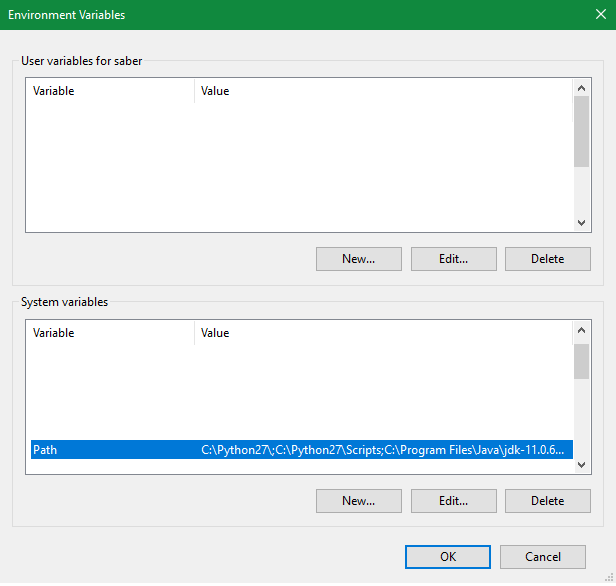
\includegraphics[width=0.7\textwidth]{images/1.png}
\end{center}


اما اگر سیستم عامل لینوکس دارید با توجه به توزیع مورد استفاده می‌توانید از گوگل بهره مند شوید:) (این \href{https://linuxize.com/post/install-java-on-ubuntu-18-04/}{\textcolor{blue}{\underline{{روش}}}} برای اوبونتو تست شده است.)


\end{itemize}

\newpage

\section*{{\titr نکات}}
\addcontentsline{toc}{section}{{\fehrestContent نکات}}

\begin{itemize}
\item
پس از اجرای سرور، در صورت نبود مشکل، آی پی و پورتی که سرور روی آن اجرا شده است در کنسول چاپ می‌شود. (اگر سرور و کلاینت روی یک کامپیوتر اجرا می‌شوند، آی پی \lr{127.0.0.1} قابل استفاده خواهد بود.)

\item
در صورت انتخاب مود دیباگ برای اجرای سرور، دستوری که هر کلاینت به سرور می‌فرستد چاپ می‌شود و همچنین هنگام قطع شدن ارتباط کلاینت از سرور تعداد کلاینت‌های آنلاین چاپ می‌شود.

\item
همچنین در مود دیباگ، پس از وصل شدن هر کلاینت به سرور یک پیام از سرور به کلاینت به شکل زیر فرستاده می‌شود. این پیام نشان دهنده این است که کلاینت با موفقیت به سرور متصل شد (به هر کلاینت متصل به بانک یک آی دی نسبت داده می‌شود که در فرایند دیباگ کردن کاربرد خواهد داشت (طبق آن چه در بالا گفته شد)‌)


\begin{latin}

\begin{lstlisting}{java}
hello "clientID"
\end{lstlisting}

\end{latin}



\item
ممکن است هنگام اجرای سرور خطاهای دیگری نظیر خطای مربوط به پورت و وصل شدن به کلاینت و … نیز چاپ شوند.

\end{itemize}

\section*{{\titr API}}
\addcontentsline{toc}{section}{{\fehrestContent API}}

\lr{API} یا \lr{Application Programming Interface} در واقع همان واسطی (\lr{interface‌}) است که به وسیله ی آن با سرور بانک ارتباط برقرار می‌کنید. در اینجا استفاده از \lr{API} به وسیله ارسال یک رشته صورت می‌گیرد و شما می‌توانید با فرمتی که در ادامه داک توضیح داده می‌شود از آن استفاده و نیاز‌های مالی فروشگاه خود را برطرف کنید. همچنین یک کد آماده در کنار فایل \lr{jar} قرار داده شده است تا شما به صورت عملی نیز با استفاده از \lr{API} بانک داده شده آشنا شوید.(‌پیشنهاد می‌شود از متدهای \href{https://docs.oracle.com/javase/7/docs/api/java/io/DataOutputStream.html#writeUTF(java.lang.String)}{\textcolor{blue}{\underline{\lr{writeUTF}}}}
 و
  \href{https://docs.oracle.com/javase/7/docs/api/java/io/DataInputStream.html#readUTF()}{\textcolor{blue}{\underline{\lr{readUTF}}}}
   برای ارسال و دریافت دستورات استفاده کنید)


\section*{{\titr ساخت اکانت}}
\addcontentsline{toc}{section}{{\fehrestContent ساخت اکانت}}


\begin{latin}

\begin{lstlisting}{java}
create_account "firstname" "lastname" "username" "password"
 "repeat_pasword"
\end{lstlisting}

\end{latin}


\begin{itemize}
\item
این متد برای ساختن حساب بانکی است.

\item
\textcolor{CustomColor}{ورودی}
 اول و دوم اسم کاربر هستند.

\item
\textcolor{CustomColor}{ورودی} سوم نام کاربری برای حساب است.

\item
\textcolor{CustomColor}{ورودی} چهارم پسورد اکانت است.

\item
\textcolor{CustomColor}{ورودی} آخر تکرار پسورد است.

\item
\textcolor{CustomColor}{خروجی} این متد یک عدد به عنوان شماره حساب است.

\item
\textcolor{CustomColor}{یک مثال}

\begin{latin}

\begin{lstlisting}{java}
create_account Bob Bobian ImBob bobword bobword
\end{lstlisting}

\end{latin}

\item
\textcolor{CustomColor}{خطاها}:

\begin{itemize}

\item
\lr{"passwords do not match"} = پسورد و تکرار آن هم خوانی ندارند.

\item
\lr{"username is not available"} = این نام کاربری قبلا استفاده شده است.

\end{itemize}


\end{itemize}

\section*{{\titr دریافت توکن}}
\addcontentsline{toc}{section}{{\fehrestContent دریافت توکن}}


\begin{latin}

\begin{lstlisting}{java}
get_token "username" "password"
\end{lstlisting}

\end{latin}

\begin{itemize}
\item
این متد برای دریافت توکن از سرور استفاده می‌شود. توکن دریافتی تا ۱ ساعت اعتبار دارد و پس از آن منقضی می‌شود، در نتیجه نیاز است که دوباره این متد صدا زده شود تا توکن تازه دریافت گردد.
\item
\textcolor{CustomColor}{ورودی} اول نام کاربری حساب بانکی است.

\item
\textcolor{CustomColor}{ورودی} دوم پسورد حساب بانکی است.

\item
\textcolor{CustomColor}{خروجی} این متد توکن است که بصورت یک رشته داده می‌شود.

\item
\textcolor{CustomColor}{خطاها}:

\begin{itemize}

\item
\lr{"invalid username or password"}

\end{itemize}


\end{itemize}

\section*{{\titr ایجاد فیش بانکی}}
\addcontentsline{toc}{section}{{\fehrestContent ایجاد فیش بانکی}}

\begin{latin}

\begin{lstlisting}{java}
create_receipt "token" "receipt_type" "money" "sourceID" "destID"
 "description"

\end{lstlisting}

\end{latin}

\begin{itemize}




\item
این متد برای ساختن فیش بانکی است. برای هر عملیات بانکی ابتدا یک فیش باید ساخته شود، سپس آن فیش را باید پرداخت کرد (عملیات آن را انجام داد).

\item
\textcolor{CustomColor}{ورودی} اول آن (یک فاصله بعد از \lr{create\_receipt}‌) ، توکن دریافتی از سرور است.

\item
\textcolor{CustomColor}{ورودی} دوم آن یکی از رشته‌های زیر است:

\begin{itemize}

\item
\lr{"deposit"}  = واریز پول به حساب
\item
\lr{"withdraw"}  = برداشت پول از حساب
\item
\lr{"move"}  = انتقال وجه

\end{itemize}

\item
\textcolor{CustomColor}{ورودی} سوم یک عدد است که مبلغ را تعیین می‌کند.

\item
\textcolor{CustomColor}{ورودی} چهارم شماره حساب مبدا است. 
\begin{itemize}
\item
برای عملیات \lr{"deposit"} این عدد 1- وارد شود.
\end{itemize}


\item
\textcolor{CustomColor}{ورودی} پنجم شماره حساب مقصد است.
\begin{itemize}
\item
برای عملیات \lr{"withdraw"} این عدد 1- وارد شود.
\end{itemize}
\item
\textcolor{CustomColor}{ورودی} آخر که اختیاری است، توضیحی در مورد تراکنش است.

\item
\textcolor{CustomColor}{خروجی} خروجی این متد یک عدد است که بیانگر ID فیش تولید شده است.
\newpage
\item
\textcolor{CustomColor}{خطاها}:
\begin{itemize}
\item
\lr{"invalid receipt type"}  = ورودی دوم نامعتبر است.
\item
\lr{"invalid money"} = عدد وارد شده برای پول صحیح نیست. (‌عدد مثبت و صحیح باید باشد)
\item
\lr{"invalid parameters passed"} = ورودی‌های داده شده از فرمت بالا پیروی نمی‌کنند.
\item
\lr{"token is invalid"} = توکن نامعتبر است. (اگر مثلا اقدام به ساخت فیش برداشت از حسابی غیر از حساب مربوط به این توکن کنید نیز این خطا داده می‌شود و بطور مشابه برای انتقال وجه)
\item
\lr{"token expired"} = توکن داده شده منقضی شده است.
\item
\lr{"source account id is invalid"}
\item
\lr{"dest account id is invalid"}
\item
\lr{"equal source and dest account"}
\item
\lr{"invalid account id"} = به جای شماره حساب معتبر، ۱- وارد شده است.
\item
\lr{"your input contains invalid characters"} = بخش توضیحات، دارای یکی از کاراکترهای خاص است (مثلا *).

\end{itemize}

\end{itemize}


\section*{{\titr دریافت گزارش تراکنش‌ها}}
\addcontentsline{toc}{section}{{\fehrestContent دریافت گزارش تراکنش‌ها}}

\begin{latin}

\begin{lstlisting}{java}
get_transactions "token" "type"

\end{lstlisting}

\end{latin}

\begin{itemize}

\item
این متد برای دریافت تاریخچه‌ی تراکنش‌ها است.
\item
\textcolor{CustomColor}{ورودی} اول توکن دریافتی از سرور است.
\item
\textcolor{CustomColor}{ورودی} دوم نوع تاریخچه را مشخص می‌کند:

\begin{itemize}
\item
\lr{"+"}  برای دریافت تاریخچه تراکنش‌هایی که مقصد آنها حساب شما (حساب مربوط به این توکن) است.
\item
\lr{"-"}  برای دریافت تاریخچه‌ی تراکنش‌هایی که مبدا آن‌ها حساب شما است.
\item
\lr{"*"}  برای دریافت تاریخچه‌ی همه‌ی تراکنش‌های مربوط به حساب شما.
\item
این ورودی همچنین می‌تواند یک عدد، بیانگر ID فیش باشد که در آن صورت آن فیش خروجی داده می‌شود.
\end{itemize}

\item
\textcolor{CustomColor}{خروجی} این تابع آرایه‌ای از فیش‌های سریالایز شده (json) خواهد بود که با "\lr{*}" از هم جدا شده‌اند. مثلا:




\begin{latin}

\begin{lstlisting}[language = json , numbers = none]
{"receiptType":"deposit",
"money":20,
"sourceAccountID":-1,
"destAccountID":10001,
"description":"",
"id":0,
"paid":1}*{"receiptType":"deposit",
"money":2000,
"sourceAccountID":-1,
"destAccountID":10001,
"description":"",
"id":0,
"paid":1}
\end{lstlisting}

\end{latin}

\begin{itemize}[label = $\star$]

\item
به فیلدهای یک فیش دقت کنید.	

\end{itemize}

\item
\textcolor{CustomColor}{خطاها}
\begin{itemize}
\item
\lr{"token is invalid"}

\item
\lr{"token expired"}

\item
\lr{"invalid receipt id"} = اگر این فیش وجود نداشته باشد یا مربوط به این حساب نباشد.


\end{itemize}

\end{itemize}



\section*{{\titr انجام تراکنش}}
\addcontentsline{toc}{section}{{\fehrestContent انجام تراکنش}}

\begin{latin}

\begin{lstlisting}{java}
pay "receiptID"

\end{lstlisting}

\end{latin}

\begin{itemize}

\item
این متد برای انجام عملیات یک فیش است (واریز ، برداشت یا انتقال وجه).

\item
\textcolor{CustomColor}{ورودی} این متد ID فیش است.

\item
\textcolor{CustomColor}{خروجی} این متد در صورت موفق بودن عملیات \lr{"done successfully"} است.
\item
\textcolor{CustomColor}{خطاها}:
\begin{itemize}
\item
\lr{"invalid receipt id"} 
\item
\lr{"receipt is paid before"} = این فیش قبلا پرداخت شده است.

\item
\lr{"source account does not have enough money"}
\item
\lr{"invalid account id"} = شماره حساب درج شده در فیش اشتباه است.


\end{itemize}



\end{itemize}


\section*{{\titr دریافت موجودی حساب}}
\addcontentsline{toc}{section}{{\fehrestContent دریافت موجودی حساب}}

\begin{latin}

\begin{lstlisting}{java}
get_balance "token"

\end{lstlisting}

\end{latin}

\begin{itemize}
\item
این متد برای گرفتن موجودی حساب است.
\item
\textcolor{CustomColor}{ورودی} آن توکن دریافتی از سرور است.
\item
\textcolor{CustomColor}{خروجی} آن موجودی حساب است.
\item
\textcolor{CustomColor}{خطاها}:
\begin{itemize}
\item
\lr{"token is invalid"}

\item
\lr{"token expired"}


\end{itemize}

\end{itemize}


\section*{{\titr قطع ارتباط با سرور}}
\addcontentsline{toc}{section}{{\fehrestContent قطع ارتباط با سرور}}

\begin{latin}

\begin{lstlisting}{java}
exit
\end{lstlisting}

\end{latin}

\begin{itemize}
\item
ارتباط کلاینت با سرور قطع می‌شود.
\end{itemize}

\subsection*{{\titr خطاهای کلی}}

\begin{itemize}

\item
\lr{"invalid input"} = ورودی وارد شده صحیح نیست.

\item
\lr{"database error"} = مشکلی در ارتباط با دیتابیس بانک وجود دارد.



\end{itemize}

\end{document}







